\subsection{\acl{halgorithm}}%
\label{subsec:halgorithm}
This section contains some \ac{hgraph}'s, a legend for is now presented.

\begin{figure}[H]
    \centering
    \begin{subfigure}{0.2\textwidth}
    \centering
    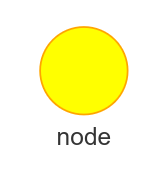
\includegraphics[width=0.7\textwidth]{figures/connecting_nodes/legend/node}
    \caption{Regular node created by the \ac{halgorithm}.\newline}%
    \end{subfigure}
    \begin{subfigure}{0.2\textwidth}
    \centering
    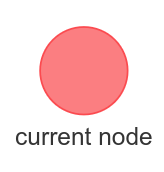
\includegraphics[width=0.7\textwidth]{figures/connecting_nodes/legend/current_node}
    \caption{Current node indicates that it's outgoing edge is now or is next to be executed.}%
    \end{subfigure}
    \begin{subfigure}{0.2\textwidth}
    \centering
    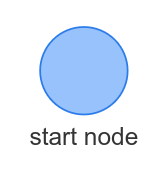
\includegraphics[width=0.7\textwidth]{figures/connecting_nodes/legend/starting_node}
    \caption{Starting node, one is generated at for every subtask.}%
    \end{subfigure}
    \begin{subfigure}{0.2\textwidth}
    \centering
    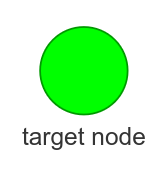
\includegraphics[width=0.7\textwidth]{figures/connecting_nodes/legend/target_node}
    \caption{Target node, one is generated for every subtask.\newline}%
    \end{subfigure}

    \begin{subfigure}{0.33\textwidth}
    \centering
    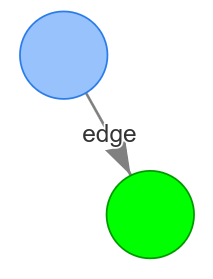
\includegraphics[width=0.7\textwidth]{figures/connecting_nodes/legend/edge}
    \caption{Edge with status IN, PE, SM, PP or EX.}%
    \end{subfigure}
    \begin{subfigure}{0.33\textwidth}
    \centering
    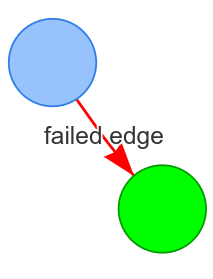
\includegraphics[width=0.7\textwidth]{figures/connecting_nodes/legend/failed_edge}
    \caption{Edge with status FAILED (FAIL)}%
    \end{subfigure}
    \begin{subfigure}{0.33\textwidth}
    \centering
    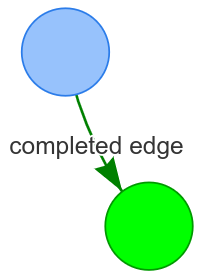
\includegraphics[width=0.7\textwidth]{figures/connecting_nodes/legend/completed_edge}
    \caption{Edge with status COMPLETED (CO)}%
    \end{subfigure}

    \caption{Legend for \ac{hgraph}'s nodes an edges}%
    \label{fig:hgraph_legend}
\end{figure}

The \ac{halgorithm}'s first step when a task is given, is to generate a start and a target node for every subtask in the task. Then, the \ac{halgorithm} tries to connect start to target nodes with a backward search, which will now be shown.\bs

\todo[inline]{search backward search, make tjhe math def, then the example}
\todo[inline]{who made this stuff, does the reader know}
\paragraph{Backward Search}%
During a backward search, edges are added pointing toward the target node (or to nodes that point toward the target node). Trying to connect the robot node through a list of succesive directed edges to a target node. If such a path has been found in the \ac{hgraph}, a hypothesis has been found and the robot can start executing edges. Two simple examples are presented a task to drive the robot to a target configuration \cref{fig:robot_drive_hgraph} and a task to push an object to a target configuration in \cref{fig:robot_push_hgraph}.\bs

\begin{figure}[H]
    \centering
    \begin{subfigure}{.3\textwidth}
    \centering
    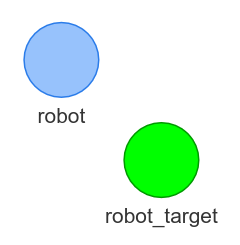
\includegraphics[width=0.7\textwidth]{figures/connecting_nodes/robot_to_target/robot_to_target}
    \end{subfigure}
    \begin{subfigure}{.3\textwidth}
    \centering
    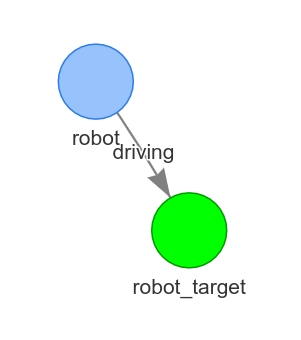
\includegraphics[width=0.9\textwidth]{figures/connecting_nodes/robot_to_target/robot_drive_target}
    \end{subfigure}
    \begin{subfigure}{.3\textwidth}
    \centering
    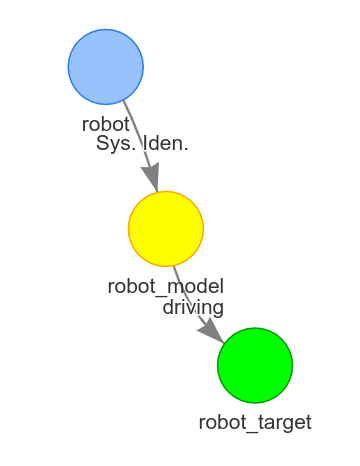
\includegraphics[width=\textwidth]{figures/connecting_nodes/robot_to_target/robot_iden_drive_target}
    \end{subfigure}
    \hfill
    \caption{\ac{hgraph} for driving the robot to target configuration}%
    \label{fig:robot_drive_hgraph}
\end{figure}

Since the robot does not yet have a system model of itself, it is forced to perform system identification before it can drive to the specified target configuration. The following figure displays succesfully executing the hypothesis found in \cref{fig:robot_drive_hgraph}.\bs

\begin{figure}[H]
    \centering
    \begin{subfigure}{.3\textwidth}
    \centering
    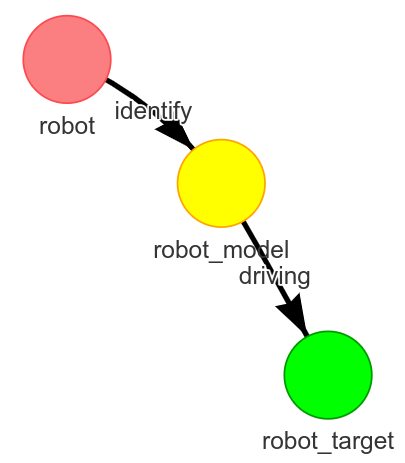
\includegraphics[width=0.8\textwidth]{figures/connecting_nodes/robot_to_target/execute_robot_to_target_1}
    \caption{}%
    \end{subfigure}
    \begin{subfigure}{.3\textwidth}
    \centering
    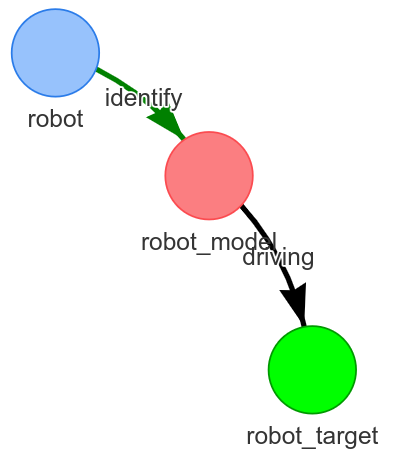
\includegraphics[width=0.8\textwidth]{figures/connecting_nodes/robot_to_target/execute_robot_to_target_2}
    \caption{}%
    \end{subfigure}
    \begin{subfigure}{.3\textwidth}
    \centering
    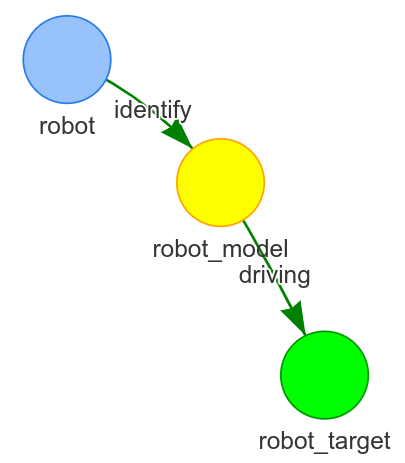
\includegraphics[width=0.8\textwidth]{figures/connecting_nodes/robot_to_target/execute_robot_to_target_3}
    \caption{}%
    \end{subfigure}
    \caption{Executing the hypothesis from \cref{fig:robot_drive_hgraph}.}
    \label{fig:execute_robot_to_target}
\end{figure}

Upcoming figure will display the hypothesis generated to push an object to a target position. Both generating a hypothesis and executing the hypothesis are intertwined, this is because information should first be collected from the environment before a feasible hypothesis is generated. An example is the \textit{best\_push\_position}, which can be found after manipulation planning for the pushing edge is completed, for motion planning to complete a system model is required, thus the corresponding system identification edge should be completed before manipulation planning can start. 

\begin{figure}[H]
    \centering
    \begin{subfigure}{.3\textwidth}
    \centering
    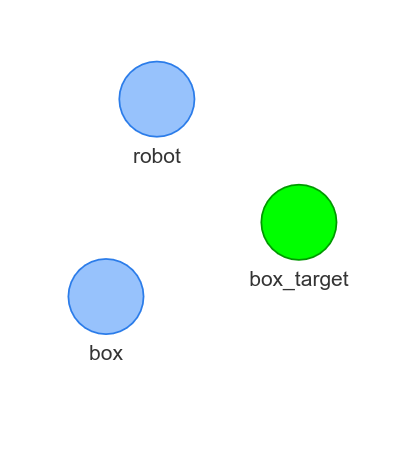
\includegraphics[width=0.8\textwidth]{figures/connecting_nodes/robot_push/robot_push_1}
    \caption{}
    \end{subfigure}
    \begin{subfigure}{.3\textwidth}
    \centering
    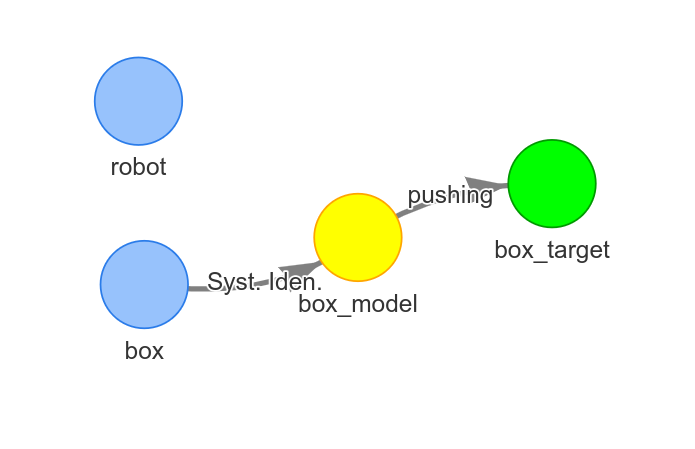
\includegraphics[width=1.1\textwidth]{figures/connecting_nodes/robot_push/robot_push_2}
    \caption{}\label{subfig:robot_push_2}
    \end{subfigure}
    \begin{subfigure}{.3\textwidth}
    \centering
    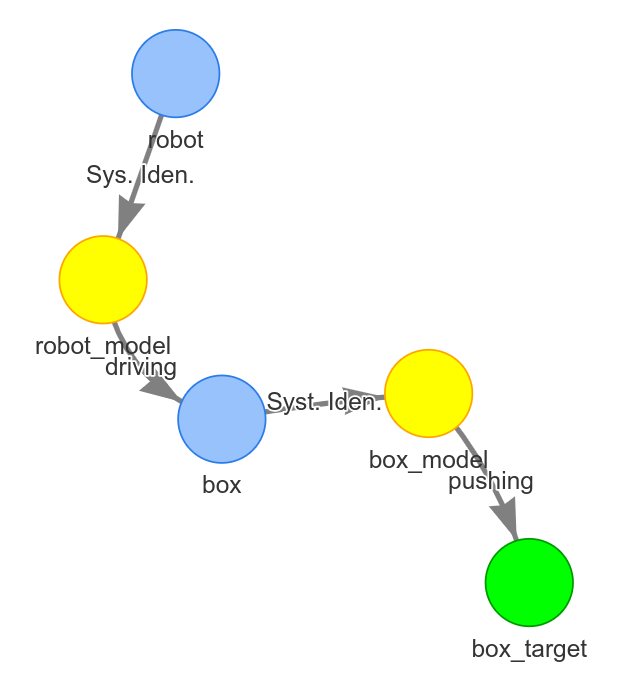
\includegraphics[width=1\textwidth]{figures/connecting_nodes/robot_push/robot_push_3}
    \caption{}\label{subfig:robot_push_3}
    \end{subfigure}

    \begin{subfigure}{.3\textwidth}
    \centering
    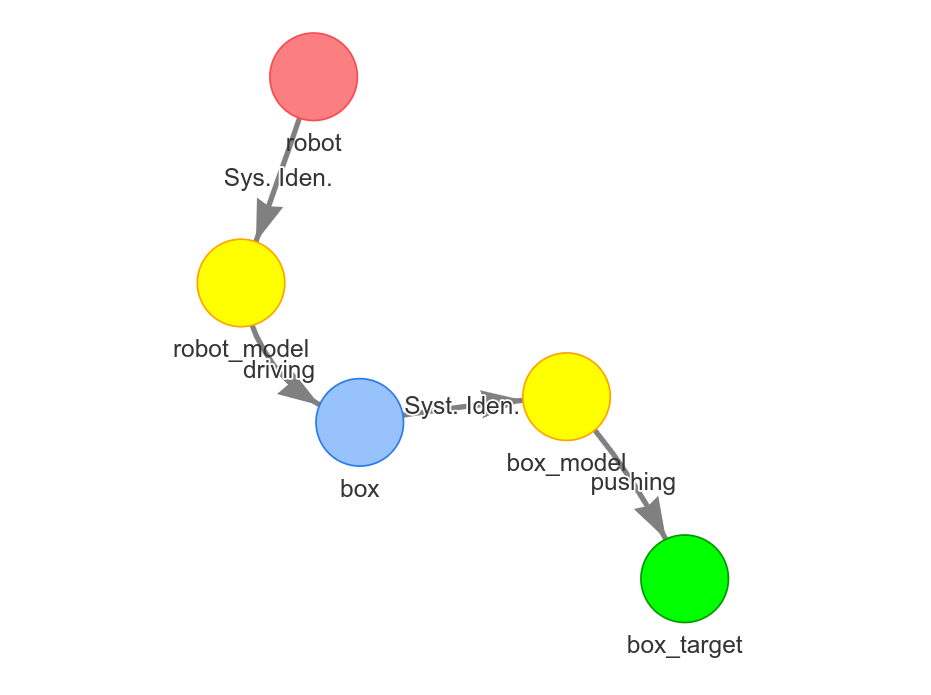
\includegraphics[width=1\textwidth]{figures/connecting_nodes/robot_push/robot_push_4}
    \caption{}\label{subfig:robot_push_4}
    \end{subfigure}
    \begin{subfigure}{.3\textwidth}
    \centering
    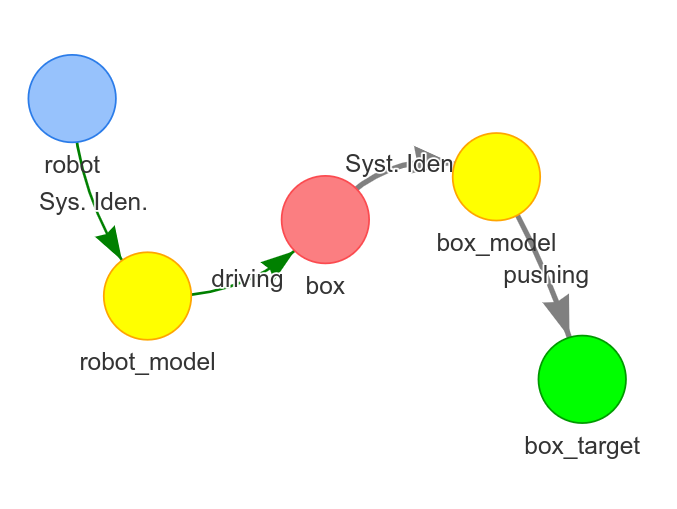
\includegraphics[width=1.05\textwidth]{figures/connecting_nodes/robot_push/robot_push_5}
    \caption{}\label{subfig:robot_push_5}
    \end{subfigure}
    \begin{subfigure}{.3\textwidth}
    \centering
    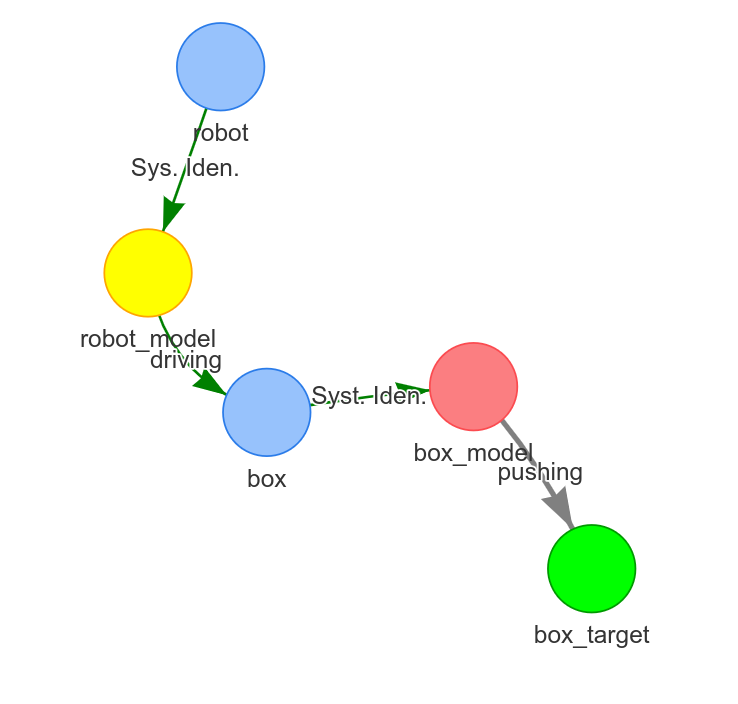
\includegraphics[width=1.05\textwidth]{figures/connecting_nodes/robot_push/robot_push_6}
    \caption{}\label{subfig:robot_push_6}
    \end{subfigure}

    \begin{subfigure}{.3\textwidth}
    \centering
    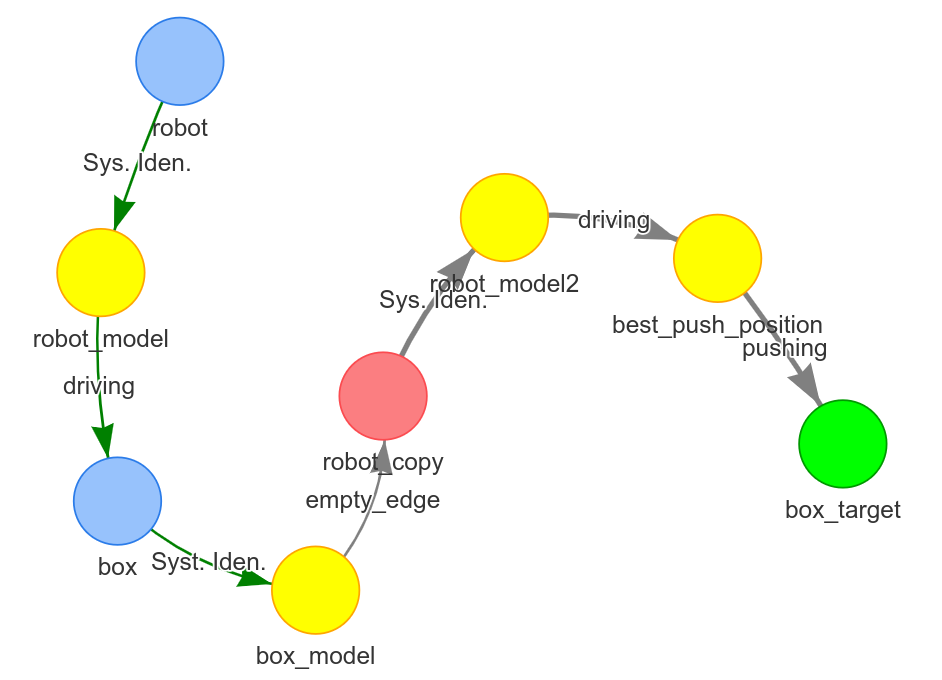
\includegraphics[width=1\textwidth]{figures/connecting_nodes/robot_push/robot_push_7}
    \caption{}\label{subfig:robot_push_7}
    \end{subfigure}
    \begin{subfigure}{.3\textwidth}
    \centering
    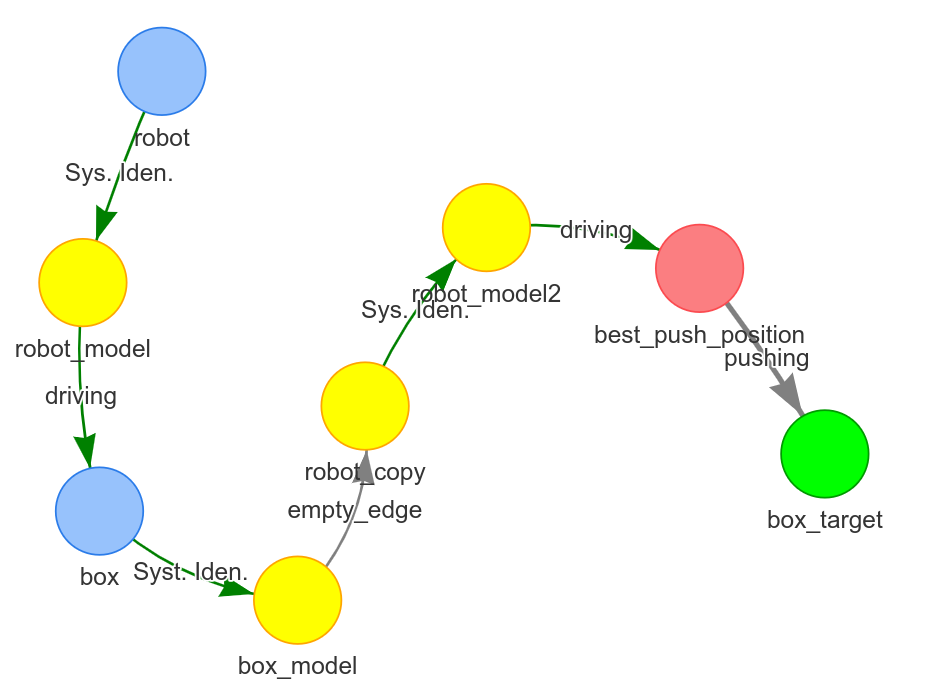
\includegraphics[width=1.05\textwidth]{figures/connecting_nodes/robot_push/robot_push_8}
    \caption{}\label{subfig:robot_push_8}
    \end{subfigure}
    \begin{subfigure}{.3\textwidth}
    \centering
    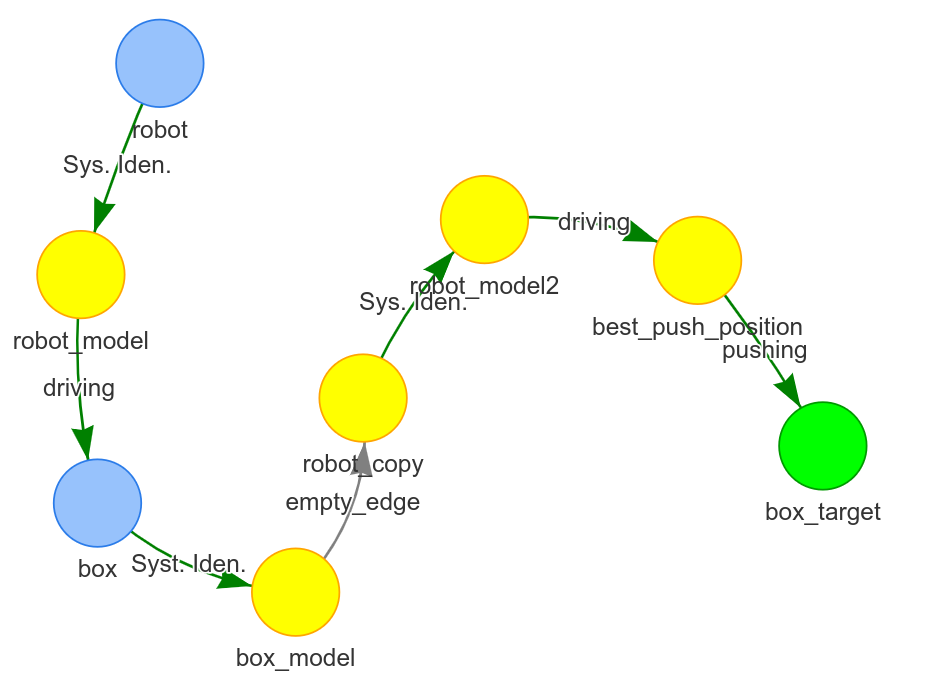
\includegraphics[width=1.05\textwidth]{figures/connecting_nodes/robot_push/robot_push_9}
    \caption{}\label{subfig:robot_push_9}
    \end{subfigure}
    \caption{\ac{hgraph} for pushing the green box to the target configuration}%
    \label{fig:robot_push_hgraph}
\end{figure}
\todo[inline]{put the current node in the figure above}
Especially in \cref{subfig:robot_push_2,subfig:robot_push_3} it is clearly visible that the \ac{halgorithm} searches from target node to robot node. \Cref{fig:robot_push_hgraph} is extensive because some steps could be skipped. First, identifying a system model for the robot twice, see \cref{subfig:robot_push_6}, if the system model from edge Sys. Iden. pointing toward node robot\_model is reused, then the edge Sys. Iden. pointing toward robot\_model\_2 would be unnecessary. Second, if system models would already be availeble for driving the robot and pushing the green box, no single system identification edge would be required.\bs

\paragraph{Encountering a Blocked Path}%
During propagation of an edge's status, motion or manipulation planning occurs, when planning detects a blocking object, the path must first be freed. The procedure can be seen in \cref{fig:free_path}.\bs

\begin{figure}[H]
    \centering
    \begin{subfigure}{.3\textwidth}
    \centering
    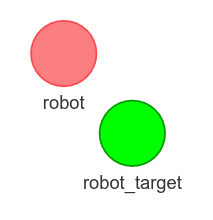
\includegraphics[width=0.5\textwidth]{figures/connecting_nodes/blocking_obj/blocking_obj_1}
    \caption{}
    \end{subfigure}
    \begin{subfigure}{.3\textwidth}
    \centering
    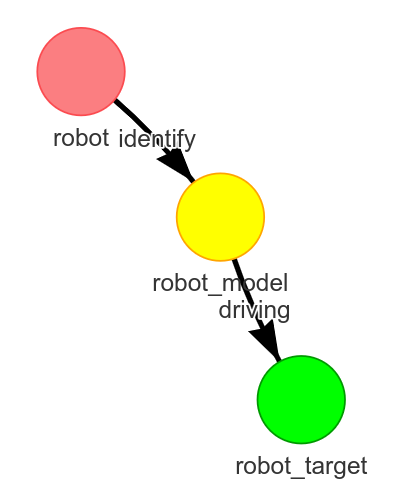
\includegraphics[width=\textwidth]{figures/connecting_nodes/blocking_obj/blocking_obj_2}
    \caption{}\label{subfig:blocking_obj_2}
    \end{subfigure}
    \begin{subfigure}{.3\textwidth}
    \centering
    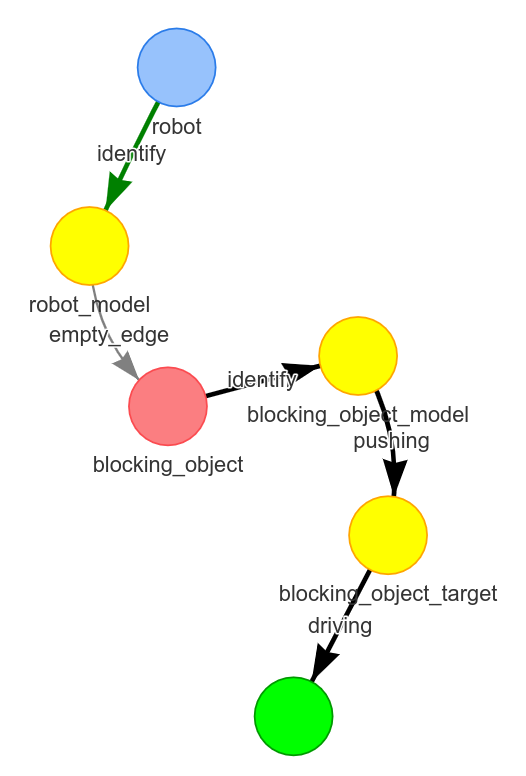
\includegraphics[width=\textwidth]{figures/connecting_nodes/blocking_obj/blocking_obj_3}
    \caption{}\label{subfig:blocking_obj_3}
    \end{subfigure}

    \begin{subfigure}{.3\textwidth}
    \centering
    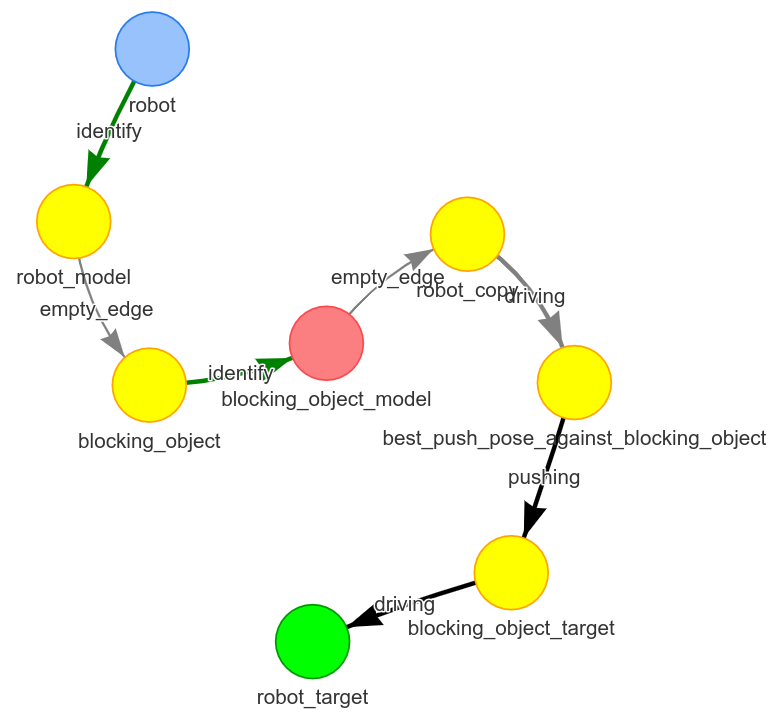
\includegraphics[width=1.3\textwidth]{figures/connecting_nodes/blocking_obj/blocking_obj_4}
    \caption{}\label{subfig:blocking_obj_4}
    \end{subfigure}
    \begin{subfigure}{.3\textwidth}
    \centering
    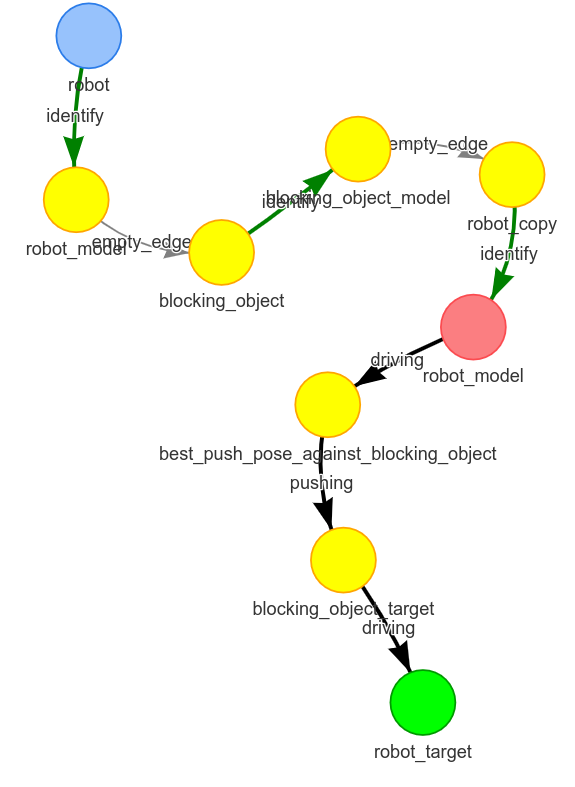
\includegraphics[width=\textwidth]{figures/connecting_nodes/blocking_obj/blocking_obj_5}
    \caption{}\label{subfig:blocking_obj_5}
    \end{subfigure}
    \begin{subfigure}{.3\textwidth}
    \centering
    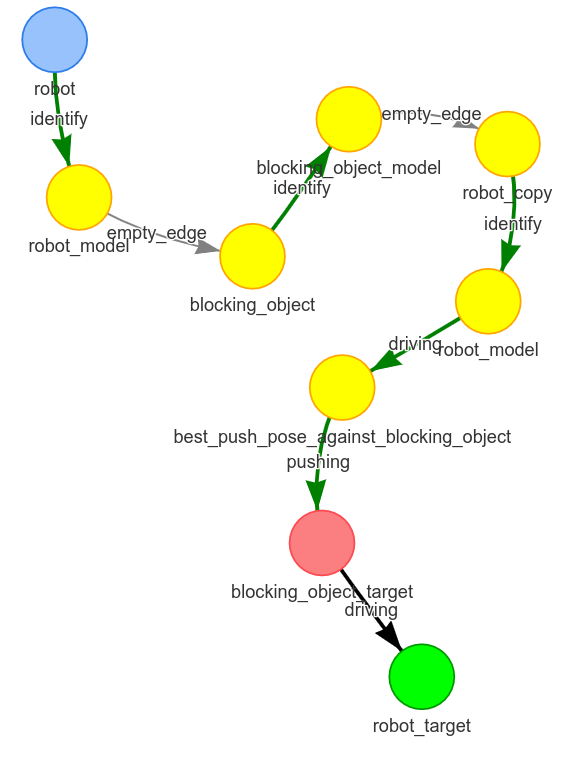
\includegraphics[width=\textwidth]{figures/connecting_nodes/blocking_obj/blocking_obj_6}
    \caption{}\label{subfig:blocking_obj_6}
    \end{subfigure}
    \caption{\ac{hgraph} for driving to target configuration and encountering a blocked path}%
    \label{fig:blocking_obj_hgraph}
\end{figure}

\paragraph{Encountering Failure}%
 Apart from blocking objects that can be detected during planning, faults and failures can occur. If during the propagation of an edge's status any kind of failure arises, the failed edge and corresponding edges are marked as failed. Equally during execution, if a fault is detected, the execution halts and the edge and corresponding edges are marked as \quotes{failed}, the procedure can be seen in \cref{subsubsec:failed_edges}.\bs


\begin{figure}[H]
    \centering
    \begin{subfigure}{.3\textwidth}
    \centering
    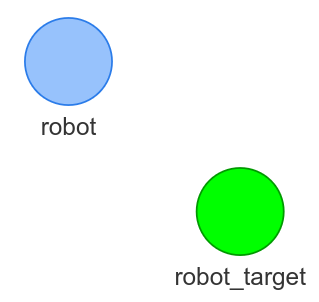
\includegraphics[width=0.8\textwidth]{figures/connecting_nodes/failure/fail_1}
    \caption{}
    \end{subfigure}
    \begin{subfigure}{.3\textwidth}
    \centering
    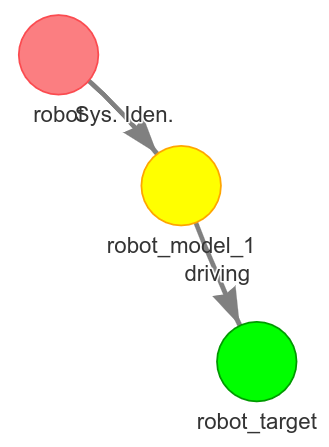
\includegraphics[width=1.1\textwidth]{figures/connecting_nodes/failure/fail_2}
    \caption{}
    \end{subfigure}
    \begin{subfigure}{.3\textwidth}
    \centering
    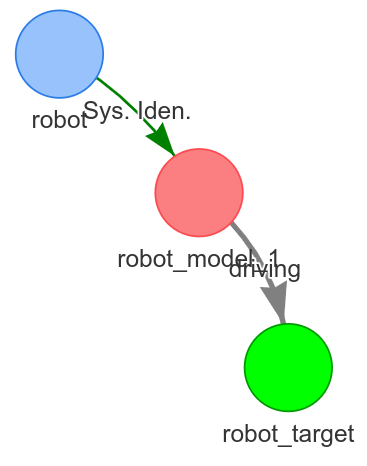
\includegraphics[width=1\textwidth]{figures/connecting_nodes/failure/fail_3}
    \caption{}
    \end{subfigure}

    \begin{subfigure}{.3\textwidth}
    \centering
    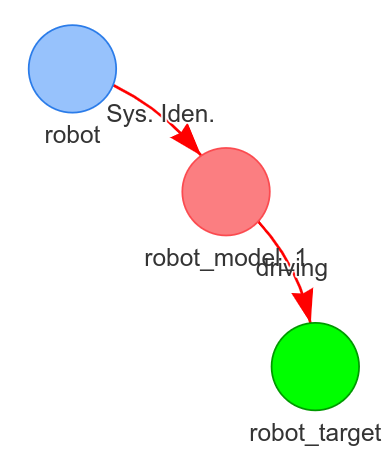
\includegraphics[width=1\textwidth]{figures/connecting_nodes/failure/fail_4}
    \caption{}
    \end{subfigure}
    \begin{subfigure}{.3\textwidth}
    \centering
    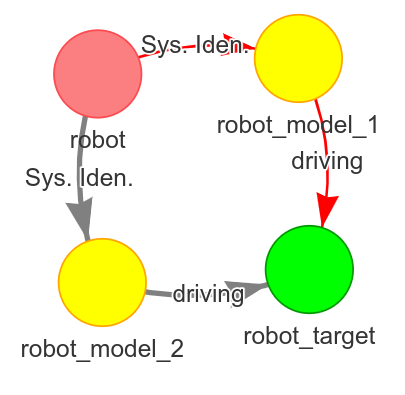
\includegraphics[width=1\textwidth]{figures/connecting_nodes/failure/fail_5}
    \caption{}
    \end{subfigure}
    \begin{subfigure}{.3\textwidth}
    \centering
    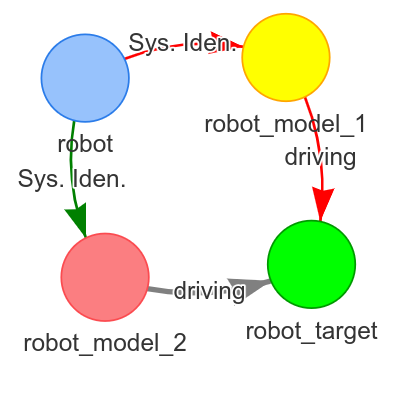
\includegraphics[width=1\textwidth]{figures/connecting_nodes/failure/fail_6}
    \caption{}
    \end{subfigure}
    \begin{subfigure}{.3\textwidth}
    \centering
    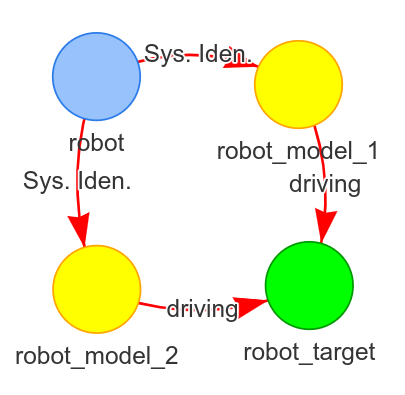
\includegraphics[width=1\textwidth]{figures/connecting_nodes/failure/fail_7}
    \caption{}
    \end{subfigure}

    \caption{todo}%
    \label{fig:failure_in_hgraph}
\end{figure}



\paragraph{The Blacklist}%
 The regeneration of failed edges must be prevented to avoid a loop of generating edges that fail and are regenerated again, \cref{subsubsec:blacklist} is dedicated to eleborating the blacklist.



